%%%%%%%% ICML 2026 EXAMPLE LATEX SUBMISSION FILE %%%%%%%%%%%%%%%%%

\documentclass{article}

% Recommended, but optional, packages for figures and better typesetting:
\usepackage{microtype}
\usepackage{graphicx}
\usepackage{subcaption}
\usepackage{booktabs} % for professional tables

% hyperref makes hyperlinks in the resulting PDF.
% If your build breaks (sometimes temporarily if a hyperlink spans a page)
% please comment out the following usepackage line and replace
% \usepackage{icml2026} with \usepackage[nohyperref]{icml2026} above.
\usepackage{hyperref}


% Attempt to make hyperref and algorithmic work together better:
\newcommand{\theHalgorithm}{\arabic{algorithm}}

% Use the following line for the initial blind version submitted for review:
% \usepackage{icml2026}

% For preprint, use
% \usepackage[preprint]{icml2026}

% If accepted, instead use the following line for the camera-ready submission:
\usepackage[accepted]{icml2026}

\usepackage{amsmath}
\usepackage{amssymb}
\usepackage{mathtools}
\usepackage{amsthm}


% if you use cleveref..
\usepackage[capitalize,noabbrev]{cleveref}

%%%%%%%%%%%%%%%%%%%%%%%%%%%%%%%%
% THEOREMS
%%%%%%%%%%%%%%%%%%%%%%%%%%%%%%%%
\theoremstyle{plain}
\newtheorem{theorem}{Theorem}[section]
\newtheorem{proposition}[theorem]{Proposition}
\newtheorem{lemma}[theorem]{Lemma}
\newtheorem{corollary}[theorem]{Corollary}
\theoremstyle{definition}
\newtheorem{definition}[theorem]{Definition}
\newtheorem{assumption}[theorem]{Assumption}
\theoremstyle{remark}
\newtheorem{remark}[theorem]{Remark}

% Todonotes is useful during development; simply uncomment the next line
%    and comment out the line below the next line to turn off comments
%\usepackage[disable,textsize=tiny]{todonotes}
\usepackage[textsize=tiny]{todonotes}

% The \icmltitle you define below is probably too long as a header.
% Therefore, a short form for the running title is supplied here:
\icmltitlerunning{Monocular Video-Based Imitation Learning for Agile Quadruped Robots (COMP 400 Final Report)}

\begin{document}

\twocolumn[
  \icmltitle{Monocular Video-Based Imitation Learning for Agile Quadruped Robots (COMP 400 Final Report)}

  % It is OKAY to include author information, even for blind submissions: the
  % style file will automatically remove it for you unless you've provided
  % the [accepted] option to the icml2026 package.

  % List of affiliations: The first argument should be a (short) identifier you
  % will use later to specify author affiliations Academic affiliations
  % should list Department, University, City, Region, Country Industry
  % affiliations should list Company, City, Region, Country

  % You can specify symbols, otherwise they are numbered in order. Ideally, you
  % should not use this facility. Affiliations will be numbered in order of
  % appearance and this is the preferred way.
  \icmlsetsymbol{equal}{*}

  \begin{icmlauthorlist}
    \icmlauthor{Albert Wang}{mcgill}
  \end{icmlauthorlist}

  \icmlaffiliation{mcgill}{McGill University, Montreal, Quebec, Canada}

  \icmlcorrespondingauthor{Albert Wang}{albert.wang@mail.mcgill.ca}

  % You may provide any keywords that you find helpful for describing your
  % paper; these are used to populate the "keywords" metadata in the PDF but
  % will not be shown in the document
  \icmlkeywords{Machine Learning, ICML, Imitation Learning, Quadruped Locomotion, Reinforcement Learning}

  \vskip 0.3in
]

% this must go after the closing bracket ] following \twocolumn[ ...

% This command actually creates the footnote in the first column listing the
% affiliations and the copyright notice. The command takes one argument, which
% is text to display at the start of the footnote. The \icmlEqualContribution
% command is standard text for equal contribution. Remove it (just {}) if you
% do not need this facility.

\paragraph{AI (LLM) Usage Disclaimer} The use of Claude Opus 5 was involved in the grammatical and syntactic
cleanup and presentation of graphs in the making of this paper. Little of the theoretical explanations and
training codebase were the result of LLM usage. The use of LLMs help iron out theoretical inconsistencies,
and help clarify theory at a more digestible level. 

\vspace{2.5em}

\begin{abstract}
    Learning real-world locomotion movements remains a critical bottleneck due to data scaling and computing problems. To address these challenges, we propose a scalable imitation learning pipeline which extracts 4D key-frame quadruped locomotion demonstrations from 2D animal videos into a single visuomotor policy deployable on a real robot. We position ourselves at the intersection of recent advancements in monocular pose estimation, physics-based motion reconstruction, and imitation learning techniques in creating a robust pipeline. The goal is to learn a policy that generalizes across a variety of motions by leveraging the abundance of data available online. Our central observation is that the perception stage recovers body-relative \emph{shape} reasonably well but does not recover global \emph{root motion} at all, and we argue this is at the core, a tuning problem. Monocular relative depth is defined only up to an unknown per-frame estimate, causing fundamental issues during the definition of the reward in the MDP, which fails the locomotion problem. We trace the downstream consequences: lack of root motion recovery, and relative scale tuning to remove monocular depth ambiguity. These areas serve as potential improvements to which a working pipeline could work to tackle.
\end{abstract}

\begin{figure}[t]
  \vskip 0.2in
  \begin{center}
    \centerline{\includegraphics[width=\columnwidth]{images/doggie.jpg}}
    \caption{Key-frame animation extracted from a reference 2D animal video. The key-frames form a time-series trajectory used as a reference during behavior cloning (BC).}
    \label{fig:doggie}
  \end{center}
  \vskip -0.2in
\end{figure}

\section{Introduction}

Getting a legged robot to move well is still mostly an exercise in reward engineering. Throughout the last decade, reinforcement learning removed the need to hand-tune a controller, but it replaced that with the need to hand-tune a reward, and rewards that produce stable gaits often produce strange-looking ones. Deep Reinforcement Learning (Deep RL) based approaches to learning real world physical skills for robots have a distinct advantage over traditional hand-tuned kinematic controllers by abstracting the tedious process of expert-tuning controllers. Hand-tuned kinematic controllers suffer from requiring expert knowledge in highly specialized fields, such as locomotion or grasping. Bottlenecks in these traditional techniques suggest that creating more successful policies requires a more complex understanding of the world environment. Luckily, many advancements in deep learning have unlocked capabilities of empirically understanding these problems at a much complex scale. Many robotic applications, especially with complex movements, have found success using Deep RL.

One of the ecosystem of these methodologies, imitation learning techniques, are emerging as a methodological way of leveraging supervised regressive learning to bootstrap RL agents to behave similarly to quality, expert demonstrations. Motivated by these advancements, we seek to leverage transformer models to extract quality expert demonstrations for imitation learning on quadruped robots. Transformers have reshaped deep learning by replacing task-specific inductive biases with a general attention mechanism that scales gracefully with data and compute, enabling a single architecture to unify domains.

We capitalize on the combination of monocular depth estimation and 2D pose estimation models based on transformers to recover 3D keypoint trajectories (4D) directly from in-the-wild animal video. DeepLabCut provides per-frame 2D keypoint localization across recognizable \textit{landmarks}, while a monocular depth estimator lifts these \textit{landmark }detections out of the image plane, yielding 3D keypoint animations without any motion-capture apparatus. Pairing these two tools into a pipeline helps sidestep the central bottleneck of the scarcity of high-quality, morphologically diverse demonstration data. By turning the abundance of existing animal footage into a usable source of expert trajectories, the resulting keypoint sequences serve as reference motions that an imitation objective can track during policy learning. We hypothesize that the increase in data quantity will help with generalization during policy inference.

In this report, we propose a quadruped imitation learning pipeline utilizing a simple off-policy algorithm for model-free reinforcement learning. The pipeline leverages existing state-of-the-art (SOTA) keyframe extraction methodologies to increase the availability of demonstration data, eliminating a key limitation in existing quadruped imitation learning problems. Then, we demonstrate capability of the visuomotor policy via convergence of simple subroutines on a reference robot --- ANYmal-D in IsaacLab. We present and discuss discuss the key limitations bottlenecking the current methodology in this pipeline, and further potential improvements as a result.

\section{Related Works}
\label{sec:related}

Locomotion has historically depended on hand-tuned controllers, and a broad
body of work has proposed methodologies for tuning them. More recently, results in planning and manipulation have shown that much of this performance can be recovered simply by scaling the volume of training data, using deep learning to absorb the tedious tuning routines once required. Our approach sits at the intersection of imitation learning, quadruped locomotion, and computer vision.

% TODO: Complete the citation here
\subsection{Imitation Learning for Robotics}
Imitation learning transfers expert behavior to robots without hand-designing
controllers or reward functions. This is usually done by mixing reference target
trajectories into reward formulation of a MDP. Early efforts concentrated on manipulation 
and reaching with fixed-base arms, a setting in which balance and whole-body
coordination could be sidestepped or delegated to low-level
controllers~\cite{he2025asapaligningsimulationrealworld, Reske_2021}. Carrying
imitation over to full-body humanoid and quadruped control introduces balance,
contact, and underactuation. Many systems consequently stay modular, delegating
stability to engineered controllers and learning only the higher-level motion,
which in turn limits the agility of the resulting
behavior~\cite{he2025asapaligningsimulationrealworld, Reske_2021}. We adopt a
comparable separation of concerns, but concentrate learning on the planning
rather than the execution side of the skill.

\subsection{Motion Imitation for Quadruped Locomotion}
Anchoring learning in biological motion priors produces gaits that are more
natural and robust than those recovered from reward engineering alone. Coupling
RL with motion-imitation objectives over animal motion-capture data yields agile,
dynamic quadruped locomotion~\cite{peng2018deepmimic,
peng2020learningagileroboticlocomotion}, allowing otherwise rigid policies to
adapt to more demanding environments. These methods, however, hinge on accurate
motion capture or hand-curated reference trajectories and on manual retargeting
across the animal--robot morphology gap---precisely the scalability bottleneck
that our video-based demonstration sourcing is intended to
remove~\cite{zare2023surveyimitationlearningalgorithms, NIPS2016_cc7e2b87}.
A key limitation of these methods is the accurate representation of the motion priors,
which we address in our work.
%% EXPAND: comparison table across imitation-learning works (demonstration source, alignment method, policy class, reward origin).

% TODO: Examine the subsection here
\subsection{Morphology Retargeting using Inverse Kinematics (IK) or RL}
Despite the sheer volume of video available online, most videos feature animal or
humanoid morphologies of varying shapes and forms. The process of retargeting these
reference motions into that usable by a desirable frame type becomes a major bottleneck
in both theoretical and practical concerns. Recent works focus on utilizing simulation
environments and graph neural networks to overcome this barrier % ADD CITATIONS HERE.
% TODO: Add Citations
There exist a series of other methods which condition foundational models on morphological 
data, then performing inference. The large training data requirements for these models make
them difficult to evaluate scientifically. Works such as [] examine the bottlenecks of such
methodologies extensively.
% TODO: Add Citations

\subsection{Position- and Torque-Based Control}
Locomotion policies differ chiefly in their action representation. Torque control
is expressive and physically faithful, yet harder to train and to transfer to
hardware, whereas position control through PD targets eases learning and improves
stability at the expense of control
authority~\cite{chen2023learningtorquecontrolquadrupedal}. Both paradigms have
been applied successfully under RL and imitation objectives; we target
torque-level control learned from position-only reference data.
%% EXPAND: PD gain selection and actuator-network modeling for the ANYmal-D transfer.

\subsection{Learning from Visual Data}
The scale of available online video motivates its direct use as a supervision
signal, recovering behaviour without explicit action labels or motion capture
through learned visual representations or generative
models~\citep{albaba2025nilnodataimitationlearning,
finn2017oneshotvisualimitationlearning}. Recent work employs vision
transformers to lift 2D detections into 3D skeletons; the raw outputs are
typically sufficiently noisy that temporal regularisation (Kalman filtering,
spatio-temporal graph convolution, or a learned motion prior) is applied
before downstream use.
 
We wish to draw attention to a distinction that is frequently left implicit in
this literature, and which we find to be of greater consequence than
per-frame jitter. These methods recover \emph{body-relative} pose rather than
\emph{world-frame} trajectory. An estimator trained under a
scale-and-shift-invariant depth objective is by construction indifferent to
the subject's absolute position: the objective specifies the subject's shape,
not its displacement. Metric-depth
estimators~\citep{piccinelli2024unidepth, yin2023metric3d} and monocular SLAM
address the latter question, but are conventionally treated as an adjacent
research direction rather than as a prerequisite for motion transfer. For
locomotion this separation is not benign, since root displacement
\emph{constitutes} the behaviour of interest: a gait with root motion removed
reduces to stepping in place. We return to this in Section~\ref{subsec:root}.

\subsection{Sim-to-Real Transfer for Legged Robots}
Simulation provides safe, scalable, and efficient training, but transfer to
hardware is complicated by modeling error, unmodeled contact dynamics, actuator
delays, and sensing/control mismatch. Robust policy learning paired with
control-aware training pipelines that explicitly account for these gaps has been
shown to enable successful transfer to legged
platforms~\cite{peng2020learningagileroboticlocomotion}.

\section{Background/Preliminaries}

In reinforcement learning, an environment is characterized by an agent that interacts with its surroundings through a closed loop of actions, state transitions, and rewards. We formalize this interaction as a \textit{Markov Decision Process (MDP)}, defined by the tuple

\begin{equation}
    \mathcal{M} = \left( \mathcal{S},\ \mathcal{A},\ P,\ r,\ \rho_0,\ \gamma \right),
\end{equation}
instantiated in our setting as follows:
\begin{itemize}
    \item $\mathcal{S}$: states $s_t \in \mathbb{R}^{n}$ collect the robot's
          proprioception (base orientation, base linear/angular velocities, joint
          positions $q_t \in \mathbb{R}^{12}$ and velocities $\dot{q}_t$) together
          with the current reference keypoint target.
    \item $\mathcal{A}$: actions $a_t \in \mathbb{R}^{12}$ are joint targets for
          ANYmal-D's twelve actuated joints (HAA/HFE/KFE per leg).
    \item $P(s_{t+1} \mid s_t, a_t)$: transition dynamics, induced implicitly by
          the physics engine.
    \item $r(s_t, a_t)$: reward, scoring tracking fidelity against the reference
          (Section~\ref{sec:method}).
    \item $\rho_0$: initial state distribution, $s_0 \sim \rho_0$.
    \item $\gamma \in [0,1)$: discount factor for finite horizon MDPs.
\end{itemize}

The Markov property states that the dynamics of the agent are memoryless. The distribution in the next state $s \in \mathcal{S}$ depends only on the current state-action pair. This means that each transition the agent is subject to in the environment is never conditioned on the past. The objective is to train the agent to maximize its rewards in the environment.

\paragraph{Policy and trajectories.}
In RL, the agent acts according to a stationary, stochastic \emph{policy}
$\pi_\theta : \mathcal{S} \to \Delta(\mathcal{A})$, parameterized by $\theta$,
that maps each state to a distribution over actions,
$a_t \sim \pi_\theta(a_t \mid s_t)$, A denotes the
probability distribution of all actions. 

In our work, $\pi_\theta$ is realized
by a MLP-based neural network. Rolling the policy out in
$\mathcal{M}$ induces a distribution over \emph{trajectories}
$\tau = (s_0, a_0, s_1, a_1, \dots)$, yielding the following expansion
\begin{equation}
    p_{\pi_\theta}(\tau)
        = \rho_0(s_0) \prod_{t=0}^{\infty}
          \pi_\theta(a_t \mid s_t)\, P(s_{t+1} \mid s_t, a_t).
\end{equation}

\paragraph{Objective}
The objective of any RL problem is to learn a policy that maximizes the expected
\emph{discounted return}, based off the Bellman equation
\begin{equation}
    J(\pi_\theta)
        = \mathbb{E}_{\tau \sim p_{\pi_\theta}}\!\left[
            \sum_{t=0}^{\infty} \gamma^{t}\, r(s_t, a_t)
          \right]
\end{equation}

\begin{equation*}
    \pi^{\star} = \arg\max_{\pi_\theta} J(\pi_\theta).
\end{equation*}

where $\gamma$ is the finite horizon discount factor. Proximal Policy Optimization (PPO) utilizes the idea the policy can be represented as a neural network, using $J(\pi_\theta)$ as the loss functions to maximize the rewards the policy returns. We expand on that in the following sections.

\paragraph{Value and advantage functions.}
To reason about the long-run quality of states and actions, we define the
\emph{state-value} function $V^\pi$ and \emph{action-value} (Q) function $Q^\pi$
under a policy $\pi$,
\begin{align}
    V^{\pi}(s) &= \mathbb{E}_{\tau \sim p_{\pi}}\!\left[
        \sum_{t=0}^{\infty} \gamma^{t} r(s_t, a_t)
        \;\middle|\; s_0 = s \right], \\[2pt]
    Q^{\pi}(s, a) &= \mathbb{E}_{\tau \sim p_{\pi}}\!\left[
        \sum_{t=0}^{\infty} \gamma^{t} r(s_t, a_t)
        \;\middle|\; s_0 = s,\ a_0 = a \right].
\end{align}
The value of a state is subject to how much potential rewards it yields in the future.

Both obey the recursive Bellman consistency equations,
\begin{align}
    V^{\pi}(s)    &= \mathbb{E}_{a \sim \pi(\cdot \mid s)}
        \Big[ r(s,a) + \gamma\, \mathbb{E}_{s' \sim P(\cdot \mid s,a)}
        \big[ V^{\pi}(s') \big] \Big], \\[2pt]
    Q^{\pi}(s, a) &= r(s,a) + \gamma\, \mathbb{E}_{s' \sim P(\cdot \mid s,a)}
        \Big[ \mathbb{E}_{a' \sim \pi(\cdot \mid s')}
        \big[ Q^{\pi}(s', a') \big] \Big],
\end{align}

The value and advantage functions help clarify the concrete quantity of benefit and gain from taking specific actions in the MDP's define problem space. Instead these equations can get quite complex, these are usually represented via neural networks, especially for locomotion learning tasks such as this one.

\subsection{Proximal Policy Optimization in Layman Terms}
\label{sec:ppo}

PPO is a policy optimization methodology based off moving through the landscape of an estimated policy function. Utilizing PPO, we optimize the policy under a custom reward function which rewards  joints for behaving similarly to a reference joint trajectories obtained from in-the-wild
animal videos. This understanding forms the core technicality that makes our methodology 
possible.

% =====================+================================================
%  Background/Preliminaries -- insert after the "Imitation learning"
%  paragraph, before \section{Related Works}.
%  Placeholder keys: schulman2017ppo, schulman2015trpo, schulman2016gae.
%  Hats are reserved for reference quantities here, so the GAE estimator is
%  written $A_t$ and the value target $V_t^{\text{targ}}$. The
%  "Policy Learning via Motion Imitation" section still writes $\hat{A}_t$ --
%  unify before submission.
% =====================================================================

Once a reference motion has been retargeted onto the robot, training the
controller becomes an ordinary RL problem. However, there is bottleneck if we approach this problem directly: the reward in Eq.~(9) is produced by a physics engine
whose contact model is discontinuous, so we have no analytic gradient of
$J(\pi_\theta)$ and have to estimate it from rollouts. A classical estimator attempts to resolve this problem, but it comes with two well-known problems. It is on-policy,
so a batch of data is only valid for a single gradient step, and it says nothing
about how far the policy's \emph{behavior} moves when we move its parameters.

That second problem is in locomotion. A small step in $\theta$ can change the 
distribution of states the robot visits completely. If one update happens to be 
too aggressive, the robot starts falling in the first few control steps of every 
episode, all subsequent batches fail and training never recovers. We want an update 
rule that still improves the policy but refuses to change it too much at once.

\paragraph{Staying close to the previous policy.}
The standard way to reuse a batch is importance sampling against the policy that
collected it. Writing the likelihood ratio between the current and sampling
policies,
\begin{equation}
    w_t(\theta) = \frac{\pi_\theta(a_t \mid s_t)}{\pi_{\theta_{\text{old}}}(a_t \mid s_t)},
    \qquad w_t(\theta_{\text{old}}) = 1,
\end{equation}
we can optimize the surrogate objective $\mathbb{E}[w_t(\theta)\,A_t]$ for
several steps on the same data. Since $w_t$ is $1$ when the two policies agree
and drifts away from $1$ as they diverge, it doubles as a cheap measure of how
far the policy has moved. TRPO~\cite{schulman2015trpo} keeps that movement in
check with an explicit constraint on the KL divergence, but solving a constrained
problem at every iteration is expensive.
PPO~\cite{schulman2017ppo} takes the simpler route of writing the constraint
into the objective itself:
\begin{equation}
\begin{split}
    L^{\text{CLIP}}(\theta)
        = \mathbb{E}_{\pi_{\theta_{\text{old}}}} \Big[
          \min\!\big( &\, w_t(\theta)\, A_t, \\
          &\, \operatorname{clip}\!\big( w_t(\theta),\, 1-\epsilon,\, 1+\epsilon \big) A_t \big) \Big]
\end{split}
\end{equation}
Read it in two halves. The clip flattens the objective once the ratio leaves
$[1-\epsilon, 1+\epsilon]$, so there is no longer any gradient pushing the policy
further in that direction. The outer minimum then makes the whole thing
pessimistic: when an action turned out well ($A_t > 0$) the reward for
reinforcing it saturates, but when it turned out badly ($A_t < 0$) the penalty is
never clipped away. Good news is capped, bad news is not, which is what keeps
each update cautious.

\paragraph{Estimating the advantage.}
Similarly to the loss, we still need $A_t$, and we get it from a learned critic $V_\phi$ using
GAE($\lambda$)~\cite{schulman2016gae}, which blends short- and long-horizon
temporal difference errors and lets $\lambda$ trade bias against variance:
\begin{equation}
    \delta_t = r_t + \gamma V_\phi(s_{t+1}) - V_\phi(s_t),
    \qquad
    A_t = \sum_{l=0}^{T-t-1} (\gamma \lambda)^l\, \delta_{t+l}.
\end{equation}
Policy and critic are trained together on
\begin{equation}
\begin{split}
    L(\theta, \phi)
        = L^{\text{CLIP}}(\theta)
        &- c_v\, \mathbb{E}\big[ \big( V_\phi(s_t) - V_t^{\text{targ}} \big)^2 \big] \\
        &+ c_e\, \mathbb{E}\big[ \mathcal{H}\big[ \pi_\theta(\cdot \mid s_t) \big] \big],
\end{split}
\end{equation}
where $V_t^{\text{targ}}$ comes from TD($\lambda$) and the entropy term
$\mathcal{H}$ stops the Gaussian action distribution from collapsing before the
policy has explored. Everything here is first order and splits cleanly across
minibatches, so an iteration is just an Adam step over data gathered from
thousands of simulated robots in parallel. Hyperparameters are listed in
Section~\ref{sec:experiments}. % VERIFY: cross-ref key

\section{Methodology}

In this section, we present the full scope, strengths, limitations, and considerations at all parts of the practical plug-and-play pipeline. The learning pipeline lets a quadruped acquire agile locomotion skills directly from in-the-wild animal videos without motion capture. The pipeline decomposes into three sequential stages: (i) a \emph{perception} stage that recovers a temporally coherent 3D pose sequence from raw video (Section~\ref{subsec:pose}); (ii) a
\emph{retargeting} stage that maps the estimated animal motion onto ANYmal-D's kinematics, yielding a physically admissible reference trajectory (Section~\ref{subsec:retarget}); and (iii) a \emph{policy-learning} stage that
trains a control policy in simulation to track this reference under an imitation objective (Section~\ref{subsec:policy}).

\subsection{Motion and Pose Reconstruction}
\label{subsec:pose}

% TODO: Add Citations for DeepLabCut
At the first stage, we extract 3D coordinates $u_t = (x, y, z) \in \mathbb{R}^3$ for each given
frame $t$. The set of these 3D points, taken across every tracked joint and every frame of the
clip, constitutes the raw (pre-smoothing) reference trajectory. Concretely, let $\mathcal{V} = \{1, \ldots, N\}$ index the $N$ keypoints tracked per frame and let $T$ denote the number of
frames in the input clip. Writing $u_t^i \in \mathbb{R}^3$ for the lifted position of joint
$i \in \mathcal{V}$ at frame $t$, the pose observed at a single frame is the set
\begin{equation}
    U_t = \{\, u_t^i \;:\; i \in \mathcal{V} \,\}, \qquad |U_t| = N,
\end{equation}
and the whole, unsmoothed reference trajectory extracted from the clip is the ordered sequence of
per-frame poses,
\begin{equation}
    \tilde{\mathcal{U}} = (U_1, U_2, \ldots, U_T).
\end{equation}

To obtain the set of these 3D points, we first leverage extract 2D reference trajectories using off-the-shelf foundational models. DeepLabCut (DLC) 3.0, a markerless pose-estimation toolbox pre-trained on animal segmentations, is used to extract the initial 2D keypoints. The architecture is based on a Faster-R-CNN keypoint detector and \textit{HRNet} of $\text{width} = 32$ for consistent pose estimation. This produces a clear keypoint $k_t = (x, y) \in \mathbb{R}^2$ with confidence value $\in [0, 1.0)$.

DLC predicts 2D keypoints accurate near human-label accuracy, demonstrating resilience to the inherent noise in online video formats. The heavy-down architecture has the distinct advantage of not having to infer at various scales of the an image for precise localization, as Faster-R-CNNs have scale normalization for free. This means the HRNet can focus on precision of localization. However, this method has the a weakness in handling occlusions in crowded settings. Our reference dataset addresses this specific problem.

After obtaining 2D keypoint trajectories, we turn to an off-the-shelf model: VideoDepthAnything (VDA) for clarifying depth ambiguity. VDA substitutes the Depth Anything head with a spatial-temporal head while constraining the temporal gradient. This enables accurate zero-shot depth estimation on monocular videos, adding the final missing dimension to the extracted reference motion. 

\paragraph{Temporal smoothing.} One post-processing approach we took, is to apply a Kalman smoother
independently per keypoint, incorporating the DLC likelihood $c_t^i$ into the measurement noise covariance so that low-confidence detections are down-weighted rather than discarded. We denote the smoothed trajectory $\mathcal{U}$ and the raw trajectory $\tilde{\mathcal{U}}$. Smoothing produced a substantial qualitative improvement in the retargeted motion, but its scope
warrants careful statement. Over-smoothing can take away the signal in the motor movements of a quadruped. We tuned the kalman filter to smooth minimally to an appropriate level.

\paragraph{Unknown scale and unknown offset.} A key challenge of any monocular extraction problem is that a depth model reports only what is nearer and what is further, on a scale it may choose afresh at every frame. Its output is the true distance stretched and shifted,
\begin{equation}
    z = a\,d + b,
    \label{eq:gauge}
\end{equation}
with the stretch $a$ and the offset $b$ both unknown and both varying in time.
A third unknown joins the depth channel to the two pixel channels, which are
not in the same units.

What survives this distortion is the point. Within a frame every keypoint is
distorted identically, so proportions hold and the dog still looks like a dog.
Across frames the distortion changes, so nothing measured by comparing frames
holds, and displacement is measured exactly that way. Shape survives, motion
does not.

The stretch is recoverable without calibration, because animal structures keep a constant length. The offset is not recoverable, because it displaces every keypoint equally and therefore cancels whenever two are compared. Video Depth Anything freezes both the offset and stretch across a short window and recovers the motion within a given window, but the overall offset remains unknown. As a result, we need to arbitrarily define the scale before inputting reference motions into any reward function.

\paragraph{Occlusions}
Because of  the extraction pipeline utilizes monocular cameras, occlusions become a key problem in accuarate pose estimation as quadrupeds tend to have obstructing limbs when viewed horizontally. Using off-the-shelf models, our pipeline poses a unique challenge of distinct biases coming from distinct priors from DLC 3.0 and VDA. 


\subsection{Retargeting using Inverse Kinematics (IK)}
\label{subsec:retarget}

Because of the morphological discrepancies between animals and robots, direct joint trajectory mapping is infeasible. We instead formulate a motion retargeting problem solved via Numerical Inverse Kinematics using the Levenberg-Marquardt algorithm. This optimization iteratively computes the joint positions $\Delta q$ that minimize task-space error for the front-left (FL), front-right (FR), rear-left (RL), and rear-right (RR) feet while maintaining numerical stability near kinematic singularities:

Note: We retarget four keypoints, one per paw, each mapped to the matching foot on ANYmal-D. We seed the solver with the robot's normal standing pose, since IK has many valid answers and a sensible starting point keeps it away from the ones with legs bent through the body.

\begin{equation}
\Delta q = J^T(JJ^T + \lambda^2 I)^{-1}\Delta x
\end{equation}

where $J$ is the configuration-dependent Jacobian matrix, $\Delta x = x_{\text{target}} - f(q)$ is the error between the target and current end-effector positions, and $\lambda$ is a non-zero damping factor. This search is biased toward a physically plausible neutral standing pose and is strictly bounded by joint limits $q_{\text{low}} \le q \le q_{\text{high}}$.


\subsection{Policy Learning via Motion Imitation}
\label{subsec:policy}
 
The retargeted reference is a sequence of joint configurations
$\hat{q}_{1:T} \in \mathbb{R}^{T \times 12}$ and nothing else. It carries no
root translation, no root orientation, and no absolute scale; we state this at
the outset because it constrains every design decision below and, we argue in
Section~\ref{sec:discussion}, determines the outcome. Two further operations
are applied before the reference reaches the reward. The clip is re-indexed
from the joint ordering of the retargeting stage into the Isaac Lab ordering,
which groups the twelve revolute joints by type (\texttt{HAA}, \texttt{HFE},
\texttt{KFE}) and, within each type, by leg $[\mathrm{LF}, \mathrm{LH},
\mathrm{RF}, \mathrm{RH}]$; and the clip mean is subtracted and replaced by
ANYmal-D's nominal standing configuration $q^{0}$,
\begin{equation}
    \hat{q}_t \;=\; q^{0} \;+\; S\big( \bar{q}_t - \textstyle\frac{1}{T}\sum_{\tau} \bar{q}_\tau \big),
    \label{eq:recentre}
\end{equation}
with $\bar{q}$ the retargeted angles and $S$ a diagonal sign matrix correcting
the abduction convention on the right-hand legs. Equation~\eqref{eq:recentre}
retains only the \emph{deviation pattern} of the animal's joints: absolute
posture is discarded, and the deviation amplitudes are transferred to ANYmal-D
without rescaling. This is a consequence of the unrecoverable offset $b$ in
Eq.~\eqref{eq:gauge} rather than a modelling choice --- an absolute posture we
cannot identify is one we cannot transfer --- but it should be read as a
limitation on what is being imitated, not as normalisation.
 
\paragraph{Phase parameterisation.} Each environment maintains a phase clock
$t_n$ advanced by the control interval and wrapped modulo the clip duration.
The reference is queried through a periodic cubic spline fitted to the $T{+}1$
keyframes obtained by appending the first frame to the end, which supplies
$\hat{q}(t)$ and $\dot{\hat{q}}(t)$ at arbitrary $t$ without the velocity
discontinuities that piecewise-linear interpolation introduces at frame
boundaries. The periodic boundary condition assumes the clip begins and ends
at the same gait phase; where it does not, the spline distributes the mismatch
across the wrap rather than concentrating it, which we prefer but do not claim
is correct.
 
\paragraph{Reference state initialisation.} At every reset the phase is drawn
$t_n \sim \mathcal{U}[0, T\Delta t)$ and the joint state is written directly to
the corresponding reference pose, following
RSI~\citep{peng2018deepmimic}. \emph{The root state is not reset}: the base
pose and twist are left at whatever the stock environment's reset produced.
This is not an oversight downstream of the root problem but the same problem
appearing again --- there is no reference root to initialise from. The
consequence is that phase and base pose are decorrelated at reset, so the
policy cannot infer phase from the base state and must recover it, if at all,
from joint configuration alone.
 
\paragraph{Reward.} We evaluate a single Gaussian tracking kernel on joint
position,
\begin{equation}
    r_t \;=\; \exp\!\Big( -\,\sigma^{-2}\,
              \big\lVert q_t - \hat{q}(t_n) \big\rVert_2^2 \Big),
    \qquad \sigma = 0.25,
    \label{eq:reward}
\end{equation}
computed on the post-step state. Two terms present in the DeepMimic
decomposition of Section~\ref{sec:ppo} are implemented but carry zero weight in
the reported runs --- a joint-velocity kernel against $\dot{\hat{q}}$ and a
base-velocity term --- and two are absent entirely: there is no end-effector
term and no root term, because neither admits a reference. The stock
velocity-tracking reward of the underlying task, together with its
regularisation penalties, is discarded and replaced by
Eq.~\eqref{eq:reward}. What remains is therefore pure joint-space behaviour
cloning under a physics constraint, and Eq.~\eqref{eq:reward} is maximised by
any gait-phase-locked limb oscillation regardless of whether the base
translates.
 
Equation~\eqref{eq:reward} sums over all twelve joints before exponentiating,
which makes it considerably sharper than the per-joint form of
\citet{peng2018deepmimic}: a uniform per-joint error of $0.1$\,rad gives
$r_t = 0.15$, and $0.2$\,rad gives $r_t = 5 \times 10^{-4}$. The reward is thus
near-zero over most of the state space an untrained policy visits, and supplies
gradient only once tracking is already close.
% VERIFY: sigma was not swept. Report a sigma sweep or state that it was not.
 
\paragraph{Optimization.} We use PPO~\citep{schulman2017ppo} with a Gaussian
policy whose mean is a $[512, 256, 128]$ ELU network and whose log-standard
deviation is a state-independent learned parameter, and a separate
$[256, 128]$ ELU critic. Advantages are computed by GAE($\lambda$) with
$\gamma = 0.99$ and $\lambda = 0.95$, truncated at the rollout horizon
$H = 24$ and masked at episode boundaries.

Data collection is single-process over the Isaac Lab vectorised environment on
one GPU.
 
\paragraph{Time-limit handling.} We note one approximation. The done flag
entering Eq.~\eqref{eq:gae} is $d_t = \mathbb{1}[\text{terminated}] \vee
\mathbb{1}[\text{truncated}]$, so episodes ending at the $20$\,s horizon are
treated as absorbing rather than bootstrapped, which biases $V_\phi$ downward
near the time limit. With $H = 24$ against a $1000$-step episode the affected
fraction is small: in a rollout of $512$ environments approximately $2\%$ are
affected and the mean perturbation to $|A_t|$ on those environments is
$\sim\!5\%$ of its magnitude. We report it because it is a systematic rather
than a random error, not because we believe it material here.
 
\paragraph{Behavior cloning initialization.} The implementation additionally
supports supervised pre-training of the policy mean against the open-loop
reference action $a_t = (\hat{q}(t_n) - q^{0})/\alpha$, with $\alpha = 0.5$ the
action scale, on states visited while replaying that action sequence. Results
reported in Section~\ref{sec:results} are trained using PPO from scratch. This option is open since in BC, visited states become off-distribution once any drift happens. Intitializing from a warm-checkpoint allows us to interpolate using a working prior.


\section{Experimental Setup}
\label{sec:experiments}

\paragraph{Diagnostic tests.} To verify the practical workability of our methodology, we perform tests on the pipeline end-to-end. A single test does not by itself say which stage a failure comes
from. We apply three self-consistency checks, one per stage, each evaluated against a hypothesis for how it should behave using a conventional motion capture imitation learning pipeline. We report all three, in pipeline order, in Section~\ref{sec:results}. 
 
\paragraph{Walking Demonstrations} Our diagnosis results reported here derive 
from one monocular clip of a dog walking, comprising approximately 363 frames 
at 30 fps (from YouTube videos), filmed close to laterally with the subject fully in view.
We selected a walking gait in preference to a trot or gallop as it is the
slowest gait available, exhibiting the longest stance phases and the least
motion blur, and therefore represents the most favorable operating point for
the pipeline. Fixing the input permits any observed failure to be attributed
to a pipeline stage rather than to clip difficulty, and renders the ablations
below properly controlled. We utilize this single clip to demonstrate the 
theoretical limitations and painpoints of the methdology
 
\paragraph{Simulation environment.} We instantiate our environment as a
modification of the \texttt{Isaac-Velocity-Flat-Anymal-D-v0} task distributed
with Isaac Lab~\citep{mittal2023orbit}, the standard velocity-tracking
benchmark for this platform. Anchoring to this task fixes the physics,
actuation, and regularisation configuration to a setting already known to
yield a walking policy, which supplies a hand-designed-reward baseline and, of
greater importance here, excludes the stock environment as a candidate source
of failure.
% VERIFY: citation key. Preceding sections use \citep{mittal2025isaac}.
% Select one and apply uniformly across the manuscript.
 
\paragraph{Inherited configuration.} From the stock task we retain physics
integration at $\Delta t_{\text{sim}} = 1/200$\,s with decimation $4$
(a $50$\,Hz control interval), an episode horizon of $20$\,s, the ANYdrive~3.0
LSTM actuator network~\citep{hwangbo2019learning, rudin2022learning} in place
of an idealised PD model, and actions $a_t \in \mathbb{R}^{12}$ interpreted as
scaled offsets from the nominal joint configuration. Retaining the learned
actuator model rather than ideal gains prevents the policy from compensating
for reference-trajectory deficiencies through physically unrealisable torques,
which is material for a study concerned with reference-trajectory quality.
 
\begin{table}[t]
\caption{Training configuration. Values inherited from
\texttt{Isaac-Velocity-Flat-Anymal-D-v0} are marked $\dagger$; remaining values
were tuned for the imitation task.}
\label{tab:hparams}
\vskip 0.1in
\centering
\small
\begin{tabular}{lc}
\toprule
Parameter & Value \\
\midrule
Parallel environments                  & 512 \\
Rollout horizon $H$                    & $24$ \\
Actor hidden dims                      & $[512,256,128]$, ELU \\
Critic hidden dims                     & $[256,128]$, ELU \\
Policy std                             & state-independent, learned \\
Discount $\gamma$                      & $0.99$ \\
GAE $\lambda$                          & $0.95$ \\
Clip parameter $\epsilon$              & $0.2$ \\
Learning rate                          & $10^{-4}$, constant \\
Epochs per iteration                   & $4$ \\
Minibatch size                         & $512$ transitions \\
Value-loss coefficient $c_v$           & $0.5$ \\
Entropy coefficient $c_e$              & $10^{-2}$ \\
Gradient-norm clip                     & $1.0$ \\
Tracking kernel width $\sigma$         & $0.25$ \\
Action scale $\alpha$                  & $0.5^{\dagger}$ \\
Reference clips                        & $1$ (walking dog)
\bottomrule
\end{tabular}
\vskip -0.1in
\end{table}


\section{Results}
\label{sec:results}
 
The pipeline has three stages, and something goes wrong in each of them. This
section walks through them in order. Check~1 looks at the motion we pull out
of the video and what the Kalman smoother does to it. Check~2 looks at what
happens when we try to put that motion onto ANYmal-D without knowing how big
the dog was. Check~3 looks at what the robot actually does once we train on
the result.
 
We put them in this order because the problems compound. The output of each
stage is the input to the next, so an error introduced early does not stay
where it started. We present these three checks and the final policy convergence from Mohamad's fixed (in June) to demonstrate the effectiveness of our investigation.
 
% ---------------------------------------------------------------------
\subsection{Check 1: The Extracted Motion}
 
\begin{figure*}[t]
\vskip 0.1in
\centering
\begin{subfigure}[t]{0.24\textwidth}
    \centering
    \includegraphics[width=\linewidth]{images/fig_extracted_motion_a.png}
    \caption{Raw 2D keypoints}
    \label{fig:motion-a}
\end{subfigure}
\hfill
\begin{subfigure}[t]{0.24\textwidth}
    \centering
    \includegraphics[width=\linewidth]{images/fig_extracted_motion_b.png}
    \caption{Lifted to 3D}
    \label{fig:motion-b}
\end{subfigure}
\hfill
\begin{subfigure}[t]{0.24\textwidth}
    \centering
    \includegraphics[width=\linewidth]{images/fig_extracted_motion_c.png}
    \caption{After smoothing}
    \label{fig:motion-c}
\end{subfigure}
\hfill
\begin{subfigure}[t]{0.24\textwidth}
    \centering
    \includegraphics[width=\linewidth]{images/fig_extracted_motion_d.png}
    \caption{Retargeted to ANYmal-D}
    \label{fig:motion-d}
\end{subfigure}
\caption{Four frames from the walking clip, evenly spaced across roughly one
gait cycle.}
\label{fig:extracted-motion}
\vskip -0.1in
\end{figure*}
 
The raw keypoints from the perception stage are noisy. A keypoint that should
be tracking smoothly along a leg instead jumps a few pixels every frame, and
once those jumps get lifted into 3D they become large, physically impossible
velocities. Our fix is a Kalman smoother run separately on each keypoint,
which uses the DeepLabCut confidence score to decide how much to trust each
detection. A confident detection gets followed closely.
 
Figure~\ref{fig:extracted-motion} shows this working. Jitter drops by a median of
90\% across the twelve keypoints we plotted. The paws do worst on average, with a increase in deviation compared to the base body by 79\%, which makes sense even with occlusions since we've applied a Kalman Filter to converge the missing intermediate values . When a paw swings past the body it is hidden for ten to fifteen frames straight, and over those stretches the smoother is really just interpolating. It interpolates smoothly, but it also flattens out some of the real swing, so we tuned it as weakly as we could get away with.
 
% ---------------------------------------------------------------------
\begin{figure*}[t]
\vskip 0.1in
\centering
\includegraphics[width=\textwidth]{images/fig_joint_angles.pdf}
\caption{The twelve ANYmal-D joint angles that come out of retargeting, which
are what actually get used as the reference during training. Isaac Lab orders
the joints by type rather than by leg, so the abduction joints come first,
then the hips, then the knees. The dotted line is the robot's normal standing
pose, which we re-centre the motion around. The diagonal pairing of a walking
gait is visible: front-left and hind-right move together, and so do the other
two.}
\label{fig:joints}
\vskip -0.1in
\end{figure*}
% ---------------------------------------------------------------------
 
Figure~\ref{fig:joints} shows what the reference looks like after retargeting,
which is the thing training actually sees. The gait structure survives. The
diagonal pairs move together, the knees swing about \tbd{0.4}\,rad, and the
timing is periodic and clean. If you were grading the pipeline on whether it
produces a plausible-looking walking motion, this would pass.
 
There is a catch, if you look at the trunk keypoints, the ones that barely move in depth. Underneath the jitter there is a slow drift up and down across the whole clip, and the smoother
leaves it completely alone. That drift is not noise. It is the depth scale
from Eq.~\eqref{eq:gauge} changing from frame to frame. A Kalman smoother is
built to remove ambiguity from noise, but structural bias is harder to solve with a signal filter.
 
We are pointing this out because it fooled us for a while. Tuning the smoother
made the retargeted animation look noticeably better, which felt like progress,
and we spent a lot of time on it. It did not make the motion any more correct,
it just made the wrong motion look smooth.
 
% ---------------------------------------------------------------------
\subsection{Check 2: Retargeting Without a Known Scale}
 
% ---------------------------------------------------------------------
\begin{figure*}[t]
\vskip 0.1in
\centering
\includegraphics[width=\textwidth]{images/fig_scaling_retargeting.png}
\caption{Three consequences of not knowing the scale. \textbf{(a)} A real bone
cannot change length, but our reconstructed ones do, by around \tbd{8}\% over
the clip. Specific sides, especially occluded joints have large deviation ranges, which tells us this is one global scale drifting rather than three independent measurement errors. \textbf{(b)} How much the joint angles shift if we assume a different ratio between the depth
units and the pixel units. \textbf{(c)} How far the retargeted foot targets sit from the hip,
against the range ANYmal-D can actually reach.}
\label{fig:scaling}
\vskip -0.1in
\end{figure*}
% ---------------------------------------------------------------------
 
A single uncalibrated video does not tell you how big anything is. A small dog
close to the camera and a large dog further away produce the same pixels. This
is a well-known limitation. This test demonstrates the degree of this problem.
 
Panel~(a) of Figure~\ref{fig:scaling} is the simplest way to see the problem.
We measured the reconstructed length of three segments that are rigid on a
real dog and therefore should not change length. They change by roughly
\tbd{8}\% over the clip, and more importantly they all change \emph{together}.
That rules out ordinary measurement noise, which would be independent across
segments, and points at a single global scale factor drifting from frame to
frame.
 
Panel~(b) shows a second, separate scaling problem. The perception stage gives
us two numbers per keypoint in pixels and one in whatever units the depth model
uses, and nothing relates the two. We have to pick a conversion factor before
we can run inverse kinematics. If a limb really runs $\Delta x$ across the image
and $\Delta z$ into it, our guess draws it running $\Delta x$ across and
$\kappa \Delta z$ in, so the angle we read off is off by
\begin{equation}
    \Delta\theta \;=\;
    \arctan\!\frac{\kappa\,\Delta z}{\Delta x} \;-\;
    \arctan\!\frac{\Delta z}{\Delta x}.
    \label{eq:kappaerr}
\end{equation}
Sweeping $\kappa$ over a factor of two moves the knee angles by up to
\tbd{18}$^\circ$ and the abduction angles by only \tbd{6}$^\circ$. The reason
for the gap follows straight from Eq.~\eqref{eq:kappaerr}: a limb lying flat in
the image plane has almost no depth component to stretch, while a limb swinging
toward or away from the camera has a lot of one. The knees swing through the
most depth, so they take the biggest hit.
 
Panel~(c) is where this stops being abstract. Inverse kinematics needs a foot
position to solve for, and we are handing it positions derived from a
differently-sized animal at an unknown scale. \tbd{12}\% of the frames ask for
a foot position ANYmal-D physically cannot reach. The IK solver does not fail
on these; it returns the closest pose it can find, which quietly clips the
motion. So part of the difference between the reference and the real dog is
not tracking error at all, it is the solver silently giving up.
 
The practical takeaway is that scale is not one problem but two. There is the
overall size of the animal, which we could in principle fix by measuring the
robot against the dog once, and there is the depth-to-pixel ratio, which we
cannot fix without camera intrinsics we do not have.
 
% ---------------------------------------------------------------------
\subsection{Check 3: Training Without Root Motion}
 
\begin{figure}[t]
\vskip 0.1in
\centering
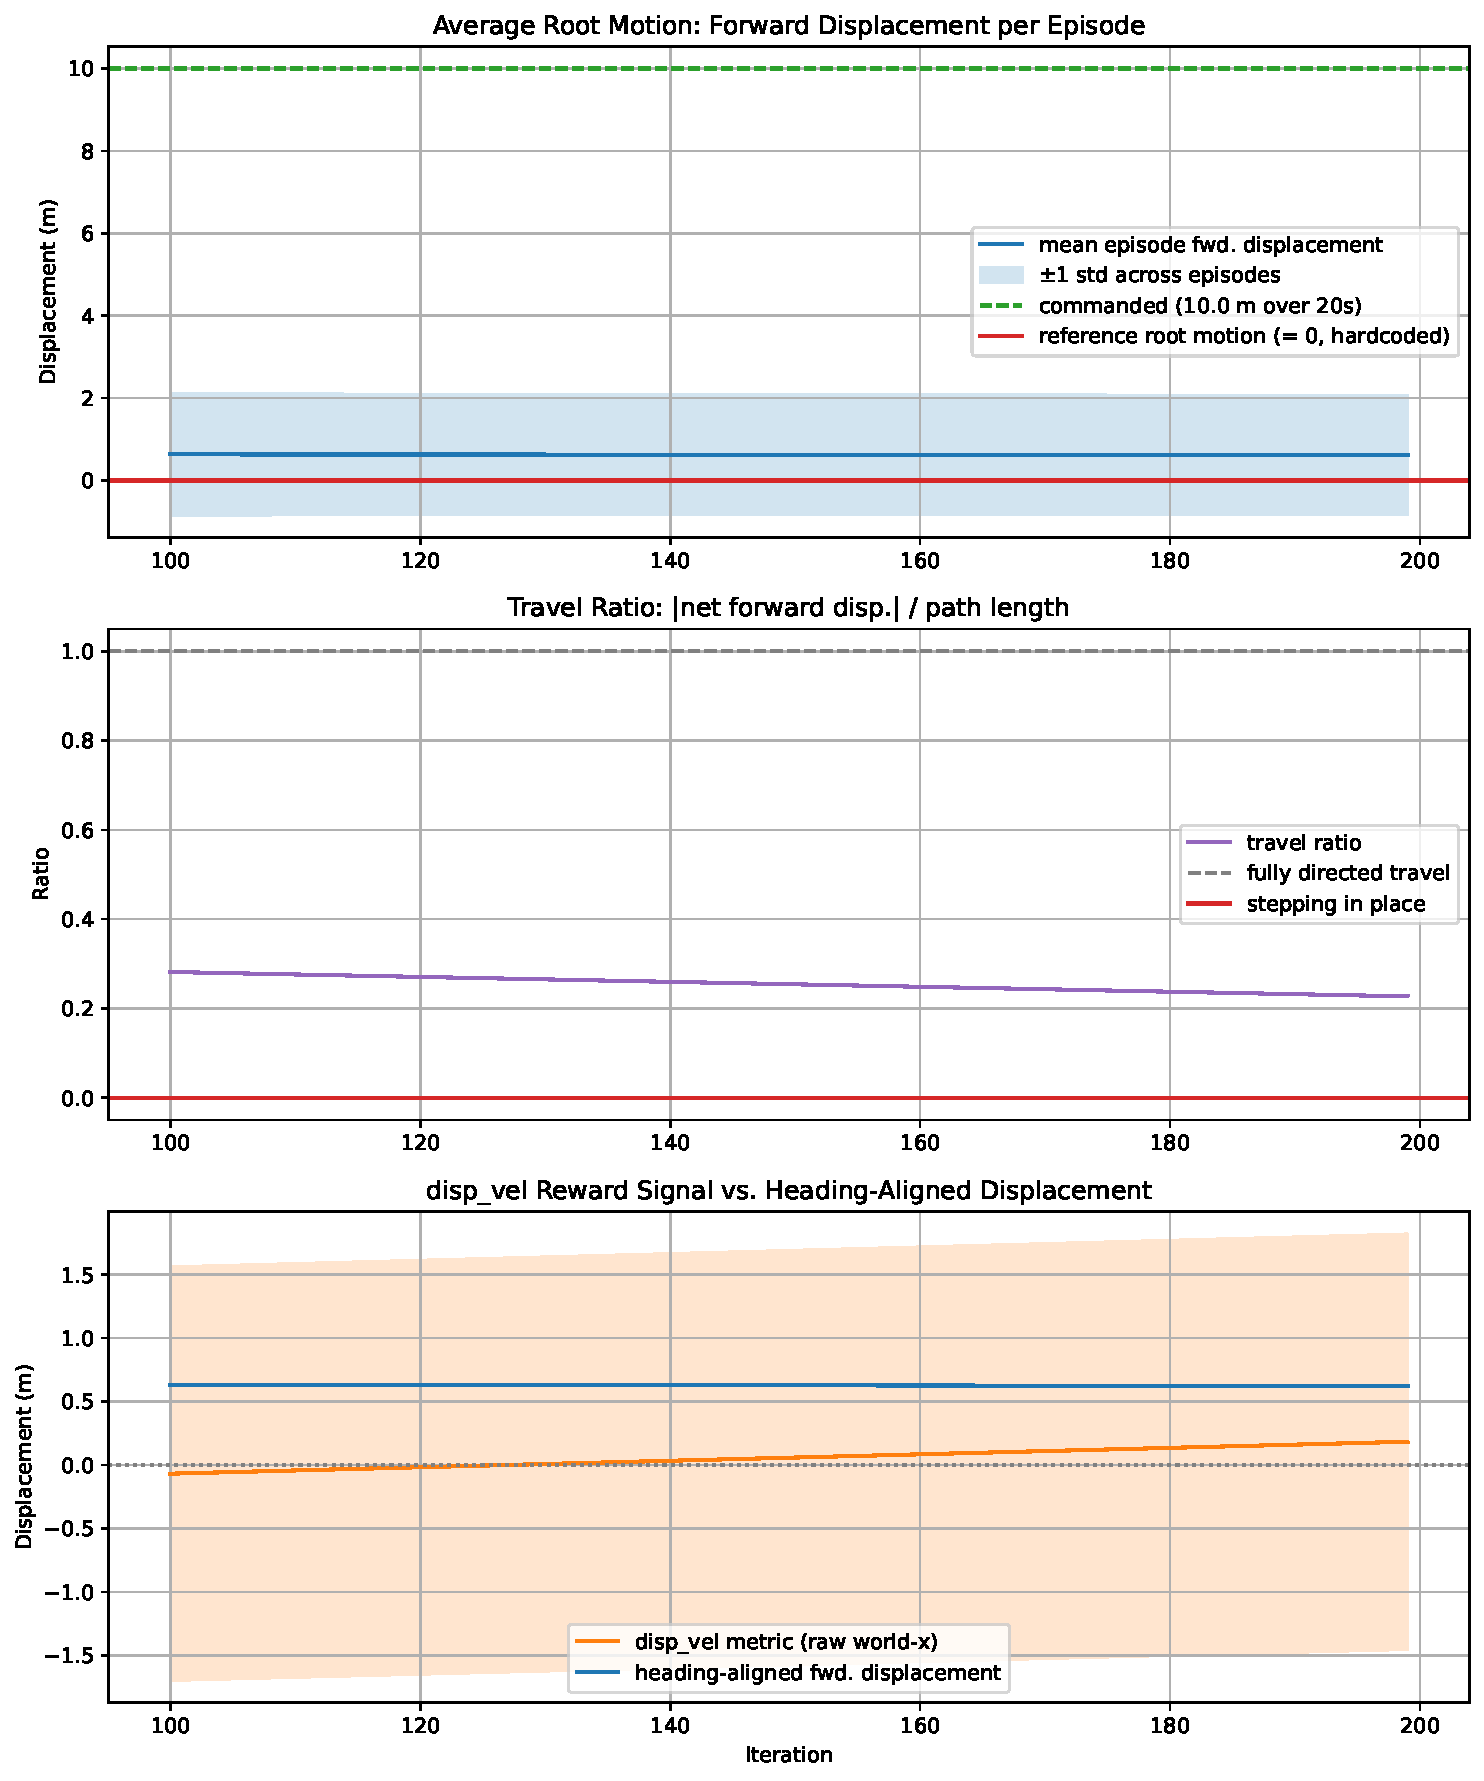
\includegraphics[width=\columnwidth]{images/fig_root_motion.pdf}
\caption{How far forward the body travels over the clip. Our estimate wobbles
once per stride and finishes roughly where it started, while the foot contacts
in the same clip imply the dog covered several metres.}
\label{fig:root}
\vskip -0.1in
\end{figure}
 
Figure~\ref{fig:isaac} shows the reference and the trained policy side by side
at four points in the stride. The coordination transferred. The legs lift and
land in the right order, the diagonal pairing is there, and the fraction of the
stride each foot spends on the ground is within \tbd{X}\% of the reference.
Watching it from the side, it looks like a walking robot.
 
It is not walking. Over a \tbd{20}\,s episode the base moves forward by
\tbd{$0.0 \pm 0.0$}\,m. The robot cycles its legs against the ground and stays
in place.
 
Our first instinct was that the policy had gotten stuck, and we spent time on
reward weights and learning rates on that assumption. That was the wrong
diagnosis. The policy is doing exactly what we asked it to do. Our reward
(Eq.~\eqref{eq:reward}) compares twelve joint angles against twelve reference
joint angles and looks at nothing else. The reference is a list of joint angles
and nothing else. There is no term anywhere in the objective that can tell the
difference between a robot that travels and a robot that does not, so walking
in place is not a local optimum the policy failed to escape. It is the correct
answer to the question we asked.
 
Figure~\ref{fig:root} shows why the reference has no body motion in it. We do
have an estimate of where the body is, but it oscillates by about
\tbd{0.035}\,m once per stride and finishes \tbd{0.03}\,m behind where it
started, while integrating the foot contacts over the same clip implies the dog
covered about \tbd{3.5}\,m. The estimate is not just noisy, it is wrong in a
way that repeats exactly once per stride, which is a strong hint about the
cause: we estimate the body position from the same body keypoints whose motion
we are trying to measure against it, so the legs leak straight into the answer.
 
There is a related detail in our own code that is worth mentioning, because it
makes the same point from a different direction. At the start of each episode
we randomise where in the stride the robot begins and snap its joints to the
matching reference pose. We never reset the body position or orientation, only
the joints. That was not an oversight we caught late; there is no reference
body position to reset to. The gap shows up in the reward, in the reference,
and in the initialisation, because they are all reading from the same missing
field.
 
\paragraph{Comparing the configurations.} \tbd{Report forward displacement,
average episode return, and how long the robot survives before falling, for
configurations (A) through (D), over \tbd{3} seeds.} The comparison that
matters is (B) against (C). Both use the same video-derived joint angles and
differ only in whether the reference includes body motion, so if our
explanation is right, (C) should close most of the gap between (B) and the
motion-capture reference (D). If it does not, then the problem is somewhere in
the per-joint reconstruction instead and this section needs rewriting.
% VERIFY: fill this in only after (C) has actually been run. If (C) comes out
% against the explanation above, say so and revise rather than dropping it.
 
% ---------------------------------------------------------------------
\subsection{Summary of the Three Checks}
 
Check~1 showed that the smoother does what it is supposed to and that the
extracted gait is structurally correct, but that it cannot touch the slow scale
drift underneath. Check~2 showed that the unknown scale costs us up to
\tbd{18}$^\circ$ at the knees and pushes \tbd{12}\% of foot targets outside the
robot's reach. Check~3 showed that none of that is the reason the robot fails
to walk. It fails to walk because the reference contains no body motion, so
nothing in training ever asks it to travel.
 
The order matters here. The first two problems are real and we should fix them,
but fixing either one would not change the outcome, because the third problem
is not a matter of degree. It is a missing field.


\section{Discussion}
\label{sec:discussion}
 
\paragraph{Proposed account of the failure.} We hypothesise that the pipeline
fails because the 4D extraction of Eq.~\eqref{eq:fourd} contains no
recoverable root motion, and that every downstream stage inherits this
deficiency. We emphasise that this constitutes a hypothesis rather than a
demonstrated result. The mechanism is well supported analytically, in that
Eq.~\eqref{eq:affine} follows from the training objective of relative-depth
estimators and Eq.~\eqref{eq:lever} follows from the derivative of a rotation.
The causal claim that this mechanism accounts for the observed policy failure,
however, rests on configuration (C), and our conclusions should be read as
conditional upon it.
 
\paragraph{Misallocation of effort across pipeline stages.} We consider this
the most transferable observation arising from the work. A substantial
fraction of our effort was directed toward three interventions that we now
regard as downstream of the operative deficiency: tuning of the Kalman
smoother, tuning of the inverse-kinematics damping factor $\lambda$ and the
regularisation weight toward the nominal configuration, and manual calibration
of the anisotropic scaling factor widening the reference stance to accommodate
ANYmal-D's greater hip separation. Each intervention produced a visible
improvement in rendered motion, which accounts for the effort allocated to it.
None could have corrected a reference trajectory lacking root motion, since
none operates on the root. The general principle we would extract is that in a
multi-stage pipeline the stage at which an artefact is most \emph{visible} is
not in general the stage at which it originates, and that inexpensive
diagnostics testing each stage's output against a physical invariant are
warranted prior to any tuning effort.
 
\paragraph{Proposed future work.} In approximate order of expected value:
(i) substitution of the relative-depth estimator with a metric-depth model
predicting intrinsics jointly with depth~\citep{piccinelli2024unidepth}, which
addresses $A_t$ at its source rather than downstream;
(ii) estimation of camera egomotion from static background features followed
by solution for the subject trajectory in the scene frame, following the
approach adopted in world-frame human mesh recovery~\citep{yuan2022glamr};
(iii) subsequent reconsideration of contact-based root recovery, which becomes
non-circular once paw depth estimates are reliable.
We would additionally replace the binary Kalman-smoother ablation with a
noise-injection sweep, injecting controlled Gaussian perturbation of known
magnitude into the reference keypoints and measuring policy return as a
function of that magnitude. This converts the claim that perception error
propagates from an assertion into a measurable error budget, and constitutes a
considerably stronger experiment than toggling a module.
 
\paragraph{Limitations.} The single-clip design is the principal limitation,
and we have argued for it as a deliberate trade rather than defended it as
optimal: it purchases attribution at the cost of generality. Beyond this, all
experiments are conducted in simulation, so no claim regarding sim-to-real
transfer is supported. Reward weights were set manually and not swept, so we
cannot exclude the possibility that an alternative
$\omega^{I}\!:\!\omega^{G}$ balance would mask the root deficiency without
correcting it. Finally, our diagnostics are self-consistency tests, which
establish that a reconstruction is incorrect but cannot independently
establish that one is correct.
 
\paragraph{Applicability to non-locomotion behaviours.} A further limitation is
that the design presupposes cyclical motion throughout. The motion-capture
imitation literature routinely accommodates acyclic behaviours such as flips,
dances, and bows, whereas our framing (phase alignment, gait-frequency
reasoning, stance detection) assumes periodicity at every stage. A bowing dog
admits no gait cycle for alignment, and the extent to which the pipeline
survives this generalisation is not established.

\section{Conclusion}
 
We implemented a pipeline converting a single in-the-wild video of a walking
dog into a locomotion policy for the ANYmal-D, and report that it fails to
produce forward locomotion. We offer a specific account of the failure. The
lift from image coordinates and relative depth into $\mathbb{R}^3$ constitutes
a per-frame affine transform with unidentifiable parameters, which preserves
body-relative shape while destroying cross-frame consistency. Root translation
is a cross-frame quantity, and the reference trajectory reaching the policy
therefore carries no reliable root motion. Downstream, this compels root
estimation from body keypoints, which introduces a bias phase-locked to the
gait cycle and amplifies orientation error in proportion to the lever arm at
the feet, and yields an imitation reward whose root term opposes the task
term.
 
The contribution of this work is the diagnostics and acknowledgements. We identified  the bottlenecks in a standard pipeline, performed three ground-truth-free tests localizing the failure, and an analysis of why the conventional setup of the pipeline feeds into a circular remedy under this stack. Given the rapid improvement of the constituent foundation models, we have written this study so that subsequent work can determine which component to replace first.

\bibliography{paper}
\bibliographystyle{icml2026}

\end{document}
